\section{Projektbeskrivelse}

Sensorsystemer I tøj, ure, telefoner, belysning og mange andre hverdagsting bliver mere og mere populære. 
Dette projekt bruges som legeplads til at interface forskellige sensor systemer ved brug af et indlejeret system.
%Målet er at kunne gøre brug af projektets resultater i fremtidig systemudvikling. 
Den specifikke case der behandles i dette project er et portabelt system der består af en GSM tranciever, en GPS reciever samt en række sensorer der kan måle temperatur, højde og barometrisk tryk. 
Data kan forespørges ved at sende en SMS der indeholder en kommando, som det fremgår af sekvensdiagrammet i figur~\ref{fig:seq-getdata}.

\begin{figure}[h]
	\centering
	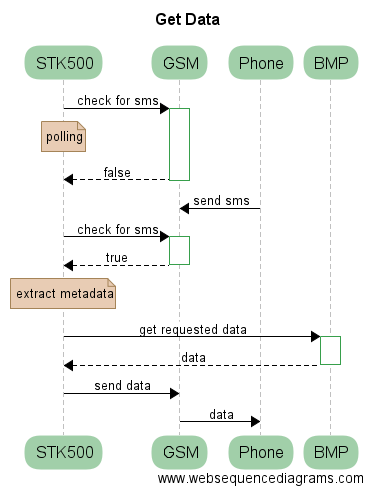
\includegraphics[width=0.7\linewidth]{figs/seq-getdata.png}
	\caption{Sekvensdiagram for hentning af data.}
	\label{fig:seq-getdata}
\end{figure}
